\documentclass{article}
\usepackage{tikz}
\usetikzlibrary{shapes.geometric, arrows}
\usepackage{graphicx} % Paquete para incluir imágenes
\usepackage{caption}  % Paquete para añadir títulos a las imágenes y diagramas

\tikzstyle{startstop} = [ellipse, minimum width=3cm, minimum height=1cm, text centered, draw=black, fill=gray!30]
\tikzstyle{process} = [rectangle, minimum width=3cm, minimum height=1cm, text centered, draw=black, fill=gray!30]
\tikzstyle{decision} = [diamond, minimum width=3cm, minimum height=1cm, text centered, draw=black, fill=gray!30]
\tikzstyle{arrow} = [thick,->,>=stealth]

\begin{document}

\title{Ciclo de Vida de la Aplicación TaskTracer}
\author{Tu Nombre}
\date{}
\maketitle

% Sección del diagrama de flujo
\section{Diagrama de Flujo}
\begin{center}
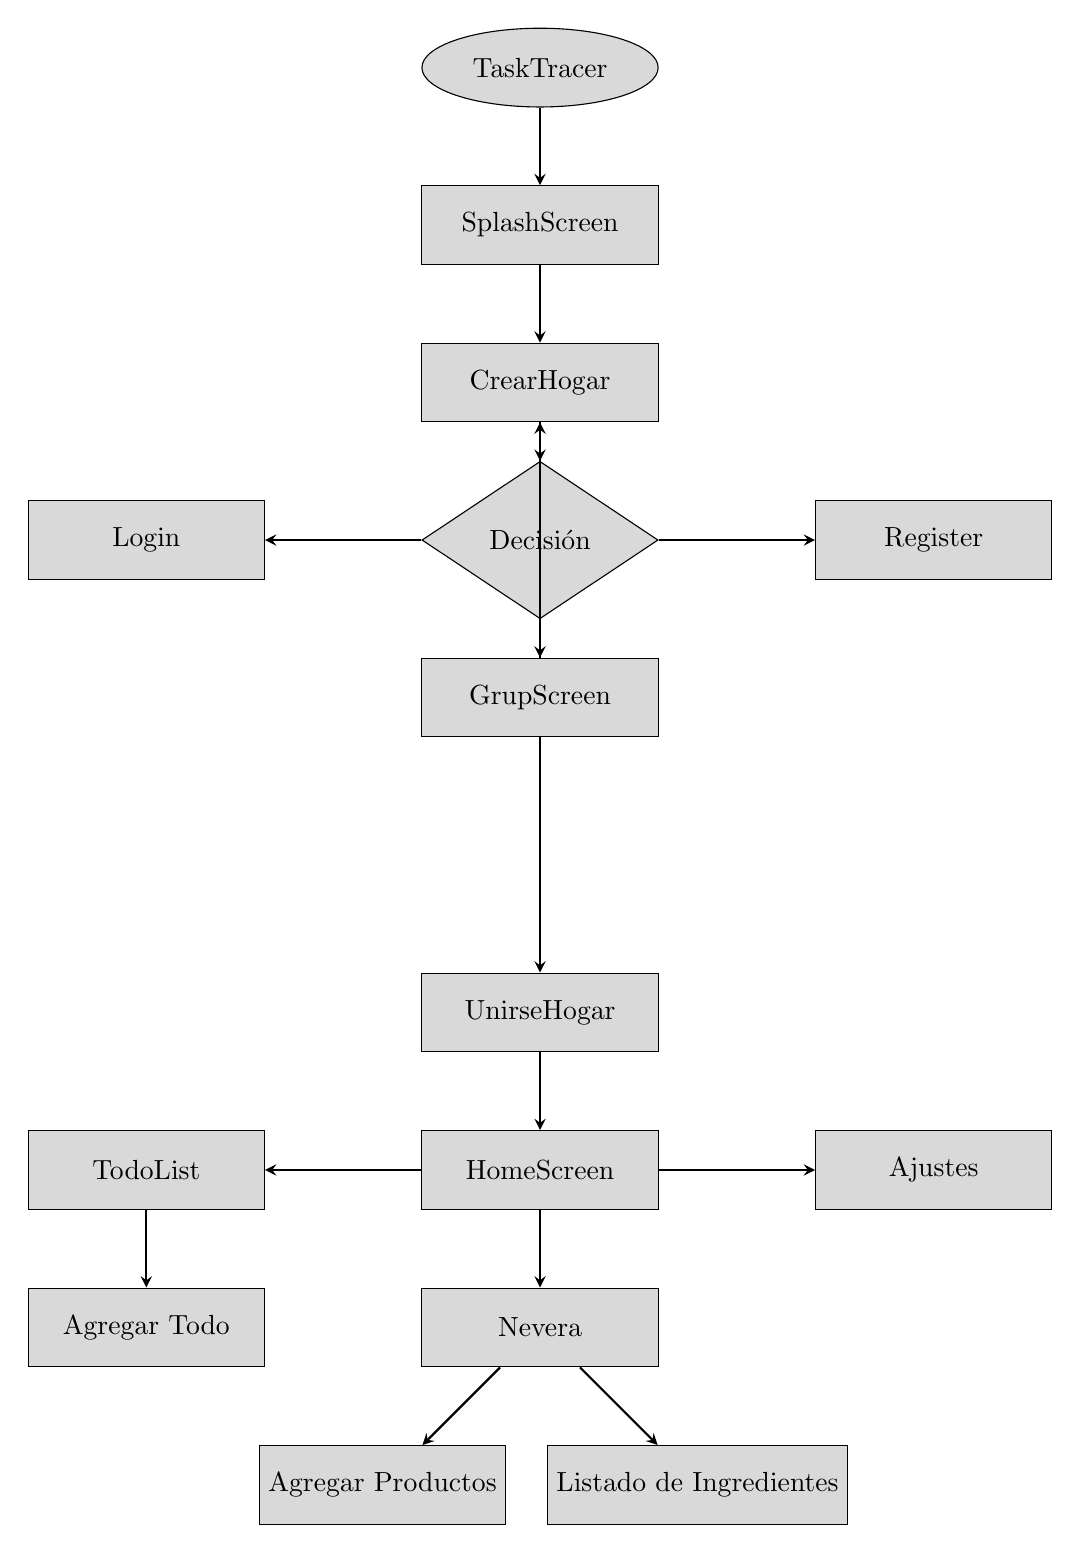
\begin{tikzpicture}[node distance=2cm]

% Nodos del diagrama
\node (start) [startstop] {TaskTracer};
\node (splash) [process, below of=start] {SplashScreen};
\node (welcome) [process, below of=splash] {Welcome};
\node (decision) [decision, below of=welcome] {Decisión};
\node (login) [process, left of=decision, xshift=-3cm] {Login};
\node (register) [process, right of=decision, xshift=3cm] {Register};
\node (grup) [process, below of=decision] {GrupScreen};
\node (creathome) [process, above of=grup, yshift=2cm] {CrearHogar}; % CrearHogar por encima de GrupScreen
\node (joinhome) [process, below of=grup, yshift=-2cm] {UnirseHogar}; % UnirseHogar por debajo de GrupScreen
\node (home) [process, below of=joinhome] {HomeScreen};
\node (todo) [process, left of=home, xshift=-3cm] {TodoList};
\node (nevera) [process, below of=home] {Nevera};
\node (ajustes) [process, right of=home, xshift=3cm] {Ajustes};
\node (addtodo) [process, below of=todo] {Agregar Todo};
\node (addprod) [process, below of=nevera, xshift=-2cm] {Agregar Productos};
\node (listprod) [process, below of=nevera, xshift=2cm] {Listado de Ingredientes};

 

% Flechas
\draw [arrow] (start) -- (splash);
\draw [arrow] (splash) -- (welcome);
\draw [arrow] (welcome) -- (decision);
\draw [arrow] (decision) -- (login);
\draw [arrow] (decision) -- (register);
\draw [arrow] (decision) -- (grup);
\draw [arrow] (grup) -- (creathome); % Flecha hacia arriba
\draw [arrow] (grup) -- (joinhome); % Flecha hacia abajo
\draw [arrow] (joinhome) -- (home);
\draw [arrow] (home) -- (todo);
\draw [arrow] (home) -- (nevera);
\draw [arrow] (home) -- (ajustes);
\draw [arrow] (todo) -- (addtodo);
\draw [arrow] (nevera) -- (addprod);
\draw [arrow] (nevera) -- (listprod);

\end{tikzpicture}
\end{center}

% Sección para añadir la imagen
\section{Imagen del Diagrama Original}
\begin{center}
\includegraphics[width=0.8\textwidth]{TFG/Captura de pantalla 2024-10-23 140334.png} % Cambia la ruta a donde tengas la imagen
\caption{Diagrama original proporcionado}
\end{center}

\end{document}
